\documentclass{beamer}
\usecolortheme{default}

\mode<presentation>
{
    \usetheme{boxes}
    \setbeamercovered{transparent}
}

%\usepackage{beamerthemesplit}
\usepackage{graphics}
\usepackage{graphicx}
\usepackage{hyperref}
\graphicspath{{../graphics/}} 
\beamertemplatenavigationsymbolsempty

\title{Determining Natural Line-Width, Quadropole and Zeeman Effects in Iron Compounds using M\"ossbauer Spectroscopy}
\author{Giacomo Resta \\ (\textit{\footnotesize gresta@mit.edu})}

\begin{document}

\frame{\titlepage}

\frame{ \frametitle{ Principle Behind M\"ossbauer Spectroscopy }
\begin{figure}
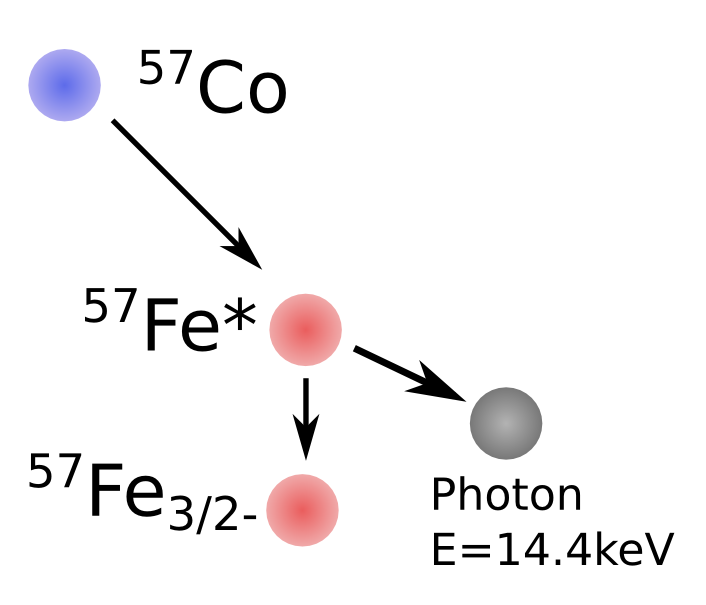
\includegraphics[width=0.5\linewidth]{principles.png}
\end{figure}
\[E' = E\left(1+v/c\right)\]
}

\frame{ \frametitle{ Equipment Setup }
\begin{figure}
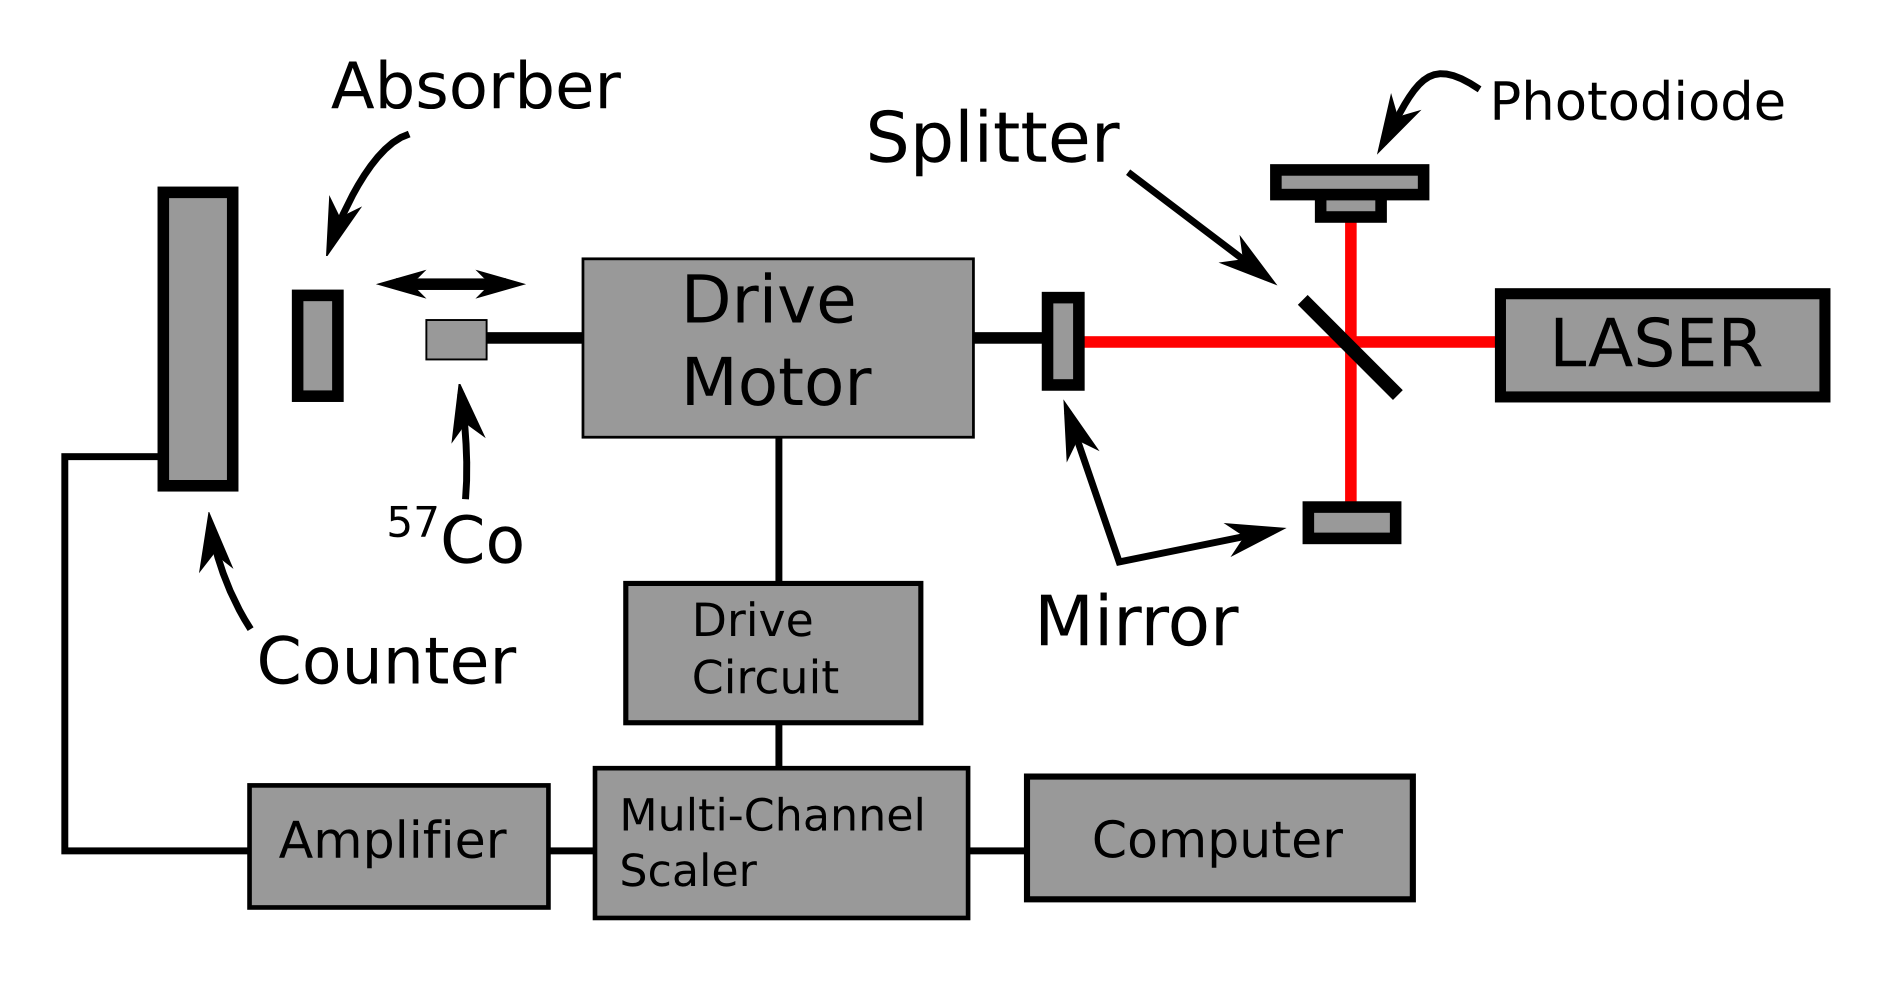
\includegraphics[width=1.0\linewidth]{setup.png}
\end{figure}
}

\frame{ \frametitle{ Absolute Velocity Calibration }
\begin{figure}
\includegraphics[width=1.0\linewidth]{vel_cal.png}
\end{figure}
}

\frame{ \frametitle{ $^{57}Fe$ Absorption Spectrum }
\begin{figure}
\includegraphics[width=1.0\linewidth]{fe_cal.png}
\end{figure}
}


\frame{ \frametitle{ Absorption Line Width and Sample Thickness }
\begin{block} {Absorption Profile,}
\[I(E) = \frac{I_0(\Gamma)^2}{(E-E_0)^2+(\Gamma)^2}\]
\end{block}
\begin{block}{Photons Transmitted (Assuming Thin Sample)}
\[C(E) = C_0\left(1-\frac{B}{(E-E_0)^2 + \Gamma^2}\right)\]
\end{block}
}

\frame{ \frametitle{ Example FWHM Fit of Absorption Line - $125[mg]$ Sample}
\begin{figure}
\includegraphics[width=1.0\linewidth]{fwhm_fit_line_width_sample_5.png}
\end{figure}
}

\frame{ \frametitle{ Determining Natural Line Width }
\begin{figure}
\includegraphics[width=1.0\linewidth]{line_width_fit.png}
\end{figure}
}

\frame{ \frametitle{ Measured Values for $^{57}Fe$ Natural Line Width }
\begin{block}{Accepted Values}
\begin{align*}
\tau_{1/2} &= 9.8\times 10^{-8}~[sec] \\ 
\Gamma &= \frac{h \ln{2}}{2 \pi \tau_{1/2}} = 4.7\times 10^{-9}~[eV]
\end{align*}
\end{block}
\begin{block}{Measured Values}
$\Gamma$: $(8.0\pm 1.5(stat))\times 10^{-9}$ [eV]

Factor of $\sigma$ Off Accepted $\Gamma$: $2.19$

$\tau_{1/2}$: $(5.7 \pm 1.1(stat))e-08$ [sec]

\vspace{10px}

FWHM $\Delta E$: $(1.60 \pm 0.3(stat))\times 10^{-8}~[eV]$

E: $(1.439999999998364 \pm 0.000000000000072(stat))\times 10^{4}$ [eV]

Fractional Width: $(1.11 \pm 0.21(stat))\times 10^{-12}$

\end{block}
}

\frame{ \frametitle{ Isomer Shift }
\begin{figure}
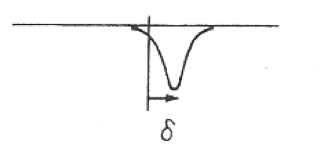
\includegraphics[width=0.4\linewidth]{iso_shift.png}
\end{figure}

\begin{align*}
\delta &= C \cdot (R_e^2-R_g^2)|\phi_s^2(0) - \phi_a^2(0)| \\
\intertext{where,}
R_e &= \text{Absorber nucleus charge radius in excited state} \\
R_g &= \text{Absorber nucleus charge radius in ground state}  \\
\phi_s &= \text{Source Electron Density}   \\
\phi_a &= \text{Absorber Electron Density}
\end{align*}
}

\frame{ \frametitle{ Absorption Spectrum of $Fe_2(SO_4)_3$ }
\begin{figure}
\includegraphics[width=1.0\linewidth]{fe2so43_fit_overview.png}
\end{figure}
}

\frame{ \frametitle{ Isomer Shift in $Fe_2(SO_4)_3$ }
\begin{figure}
\includegraphics[width=1.0\linewidth]{fe2so43_fit_iso.png}
\end{figure}
}

\frame{ \frametitle{ Quadrupole and Zeeman Effects}
\begin{block}{Quadrupole}
\begin{columns}
\begin{column}{0.5\linewidth}
    \begin{figure}
        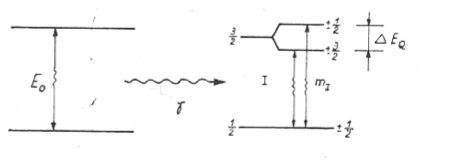
\includegraphics[width=1.0\linewidth]{quad_1.png}
    \end{figure}
\end{column}
\begin{column}{0.5\linewidth}
    \begin{figure}
        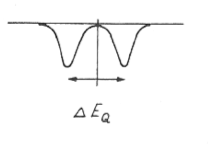
\includegraphics[width=0.5\linewidth]{quad_2.png}
    \end{figure}
\end{column}
\end{columns}
\end{block}
\begin{block}{Zeeman}
\begin{columns}
\begin{column}{0.5\linewidth}
    \begin{figure}
        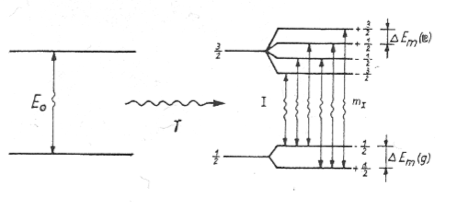
\includegraphics[width=1.0\linewidth]{zee_1.png}
    \end{figure}
\end{column}
\begin{column}{0.5\linewidth}
    \begin{figure}
        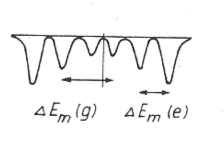
\includegraphics[width=0.5\linewidth]{zee_2.png}
    \end{figure}
\end{column}
\end{columns}
\end{block}
}

\frame{ \frametitle{ Peak Fitting Quadrupole and Zeeman Effects in $Fe_2O_3$ }
\begin{figure}
\includegraphics[width=1.0\linewidth]{fe2o3_fit.png}
\end{figure}
}

\frame{ \frametitle{ Measured Values for Quadrupole and Zeeman Effects in $Fe_2O_3$}
\begin{align*}
\Delta E_g &= (4.018 \pm 0.013(stat))e-07~[eV] \\
\Delta E_m &= (2.294 \pm 0.013(stat))e-07~[eV] \\
\Delta Q &= (9.4 \pm 1.6(stat))e-09~[eV] \\
\end{align*}
}


\frame{ \frametitle{ Measurement of the Absorption Spectrum for $Fe_3 O_4$ }
\begin{figure}
\includegraphics[width=1.0\linewidth]{fe3o4_9_fit.png}
\end{figure}
}

\frame{ \frametitle{ Chemical Structure of $Fe_3 O_4$ }
\begin{figure}
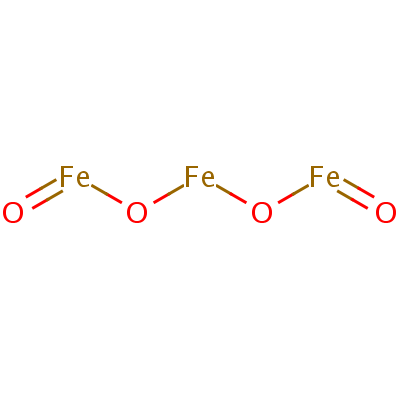
\includegraphics[width=0.5\linewidth]{fe3o4_picture.png}
\end{figure}
{\small https://www.ebi.ac.uk/chebi/}
}

\frame{ \frametitle{ Measurement of the Absorption Spectrum for $Fe_3 O_4$ }
\begin{figure}
\includegraphics[width=1.0\linewidth]{fe3o4_9_fit.png}
\end{figure}
}

\frame{ \frametitle{ Final Remarks }
\begin{itemize}
\item M\"ossbauer spectroscopy allows for fine measurements of atomic structure.   
\item We have confirmed accepted measurements for $\tau_{1/2}$ in $^{57} Fe$.
\item The technique can be applied to provide information about the chemical structure of a substance as demonstrated by our application to $Fe_3 O_4$. 
\end{itemize}
}

\frame{}

\end{document}
